\documentclass[12pt,letterpaper]{article}

%Note to Self:
%When Decommission? - after two months of feeling useless or right away?

\usepackage[utf8]{inputenc}
\usepackage[letterpaper,margin=1in]{geometry}
\usepackage{caption} % for table captions

\usepackage{amsmath} % for multi-line equations and piecewises
\usepackage{indentfirst} % to indent after a section
\usepackage{setspace}
\usepackage{times}
\usepackage{graphicx}
\usepackage{textcomp}
\usepackage{xspace}
\usepackage{verbatim} % for block comments
\usepackage{subfig} % for subfigures
\usepackage{enumitem} % for a) b) c) lists
\usepackage{tabularx}
\usepackage{cleveref}
\usepackage{xcolor}
\usepackage{soul}
\newcommand{\mathcolorbox}[2]{\colorbox{#1}{$\displaystyle #2$}}

\newcolumntype{b}{X}
\newcolumntype{s}{>{\hsize=.5\hsize}X}
\newcolumntype{m}{>{\hsize=.75\hsize}X}
\usepackage{titling}
\usepackage{minted}

\newcommand{\subtitle}[1]{%
  \posttitle{%
    \par\end{center}
    \begin{center}\large#1\end{center}
    \vskip0.5em}%
}
\usepackage{tikz}


\usetikzlibrary{shapes.geometric,arrows}
\tikzstyle{process} = [rectangle, rounded corners, minimum width=3cm, minimum height=1cm,text centered, draw=black, fill=blue!30]
\tikzstyle{arrow} = [thick,->,>=stealth]


\graphicspath{{images/}}
 
\usepackage[font={footnotesize,it}]{caption}
 



\setlength{\parindent}{15pt} % Default is 15pt.




\fontfamily{ptm}\selectfont

\title{CP1 for NPRE 501}
\author{Jin Whan Bae}
\date{2017-11-01}


\begin{document}
	
	\maketitle
	\hrule
	\onehalfspacing
	\thispagestyle{empty}

\section*{Problem Definition}

\Cref{tab:constants} lists the constants used in the problem.


\begin{table}[h]
     \centering
    \begin{tabularx}{\textwidth}{bbb}
       \hline
       Parameter & Value & [Unit] \\
       \hline
       Diamater & 6 & [cm] \\
       \textbf{Radius} & \textbf{3} & [cm] \\
       Geometry & Sphere \\
       k & 15 & [$ \frac{W}{mK} $] \\
       Density & 8000 & [$ \frac{kg}{m^3} $] \\
       Specific Heat & 500 & [$ \frac{J}{kgK} $] \\
       \textbf{$ \alpha$} & \textbf{3.75e-6} & [$ \frac{m^2}{s} $] \\
       \hline
    \end{tabularx}
    \caption {Problem Constants. Derived constants are in bold.}
    \label{tab:constants}
\end{table}

Differential Equation:
\[\frac{1}{\alpha} \cdot \frac{dT}{dt} = \frac{1}{r^2} \frac{d}{dr} r^2 \frac{dT}{dr}\]

Boundary Conditions:
\[T(0,t) = finite \quad OR \quad \frac{dT}{dr} (r = 0, t) = 0\]
\[\frac{dT}{dr} (r = R) = 0 \]

Initial Condition:
\[T(r,0) = \frac{T_0}{2} (1-\cos{(\frac{\pi \cdot r}{R})}) \]


\section*{Analytical Term Study}
For the term study, it is speculated that for higher time values,
less terms ($\beta_n$) would be needed for reasonable convergence,
since a higher time value would cause the exponential term, which has
$\beta$ in, less of a contribution. The solved equation from Appendix A
proves this mathematically:

\[\overline{T}(r,t) = \sum_{n=1}^{\infty} A_n e^{-\alpha \beta_n^2 t} sin(\beta_n r)\]

The study is conducted where different number of betas are used for each timestep.
Seven timesteps are used: $t = 0, 2, 4, 17.7, 31.1, 62.2, 75$.
A 'reasonable convergence' is met when $$ \sum_{r=0}^{R} (|r_{r}^n - r_{r}^{n+1}|) < 1e-3$$
Where n is the number of terms used for the temperature profile.

\Cref{tab:conv} organizes the `reasonable convergence` point of all timesteps.

\begin{table}[h]
     \centering
    \begin{tabular}{cc}
       \hline
       \textbf{Time [secs]} & \textbf{Number of Terms for Convergence}  \\
       \hline
       0 & 17 \\
       2 & 7 \\
       4 & 5 \\
       17.7 & 3 \\
       31.1 & 2 \\
       62.2 & 2 \\
       75 & 2 \\
       \hline
    \end{tabular}
    \caption {Timestep and number of terms for convergence.}
    \label{tab:conv}
\end{table}


As expected, as time increases, the number of terms for convergence
becomes minimal. 
\Cref{fig:0}, \ref{fig:2}, \ref{fig:4}, \ref{fig:17}, \ref{fig:31}, \ref{fig:62}, \ref{fig:75} show the 
convergence study where the temperature profile is plotted with
increasing number of terms. Note the visible difference is negligible.
Also note the y axis range change for different times.


\begin{figure}[htbp!]
  \begin{center}
    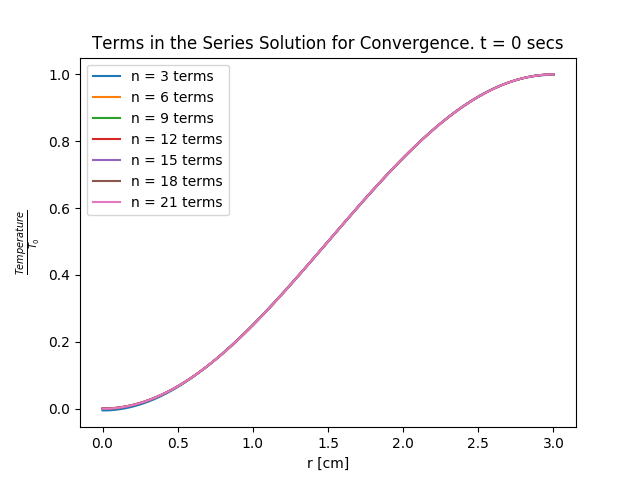
\includegraphics[scale=0.7]{terms_0.png}
  \end{center}
  \caption{Number of terms convergence study for t = 0.}
  \label{fig:0}
\end{figure}

\begin{figure}[htbp!]
  \begin{center}
    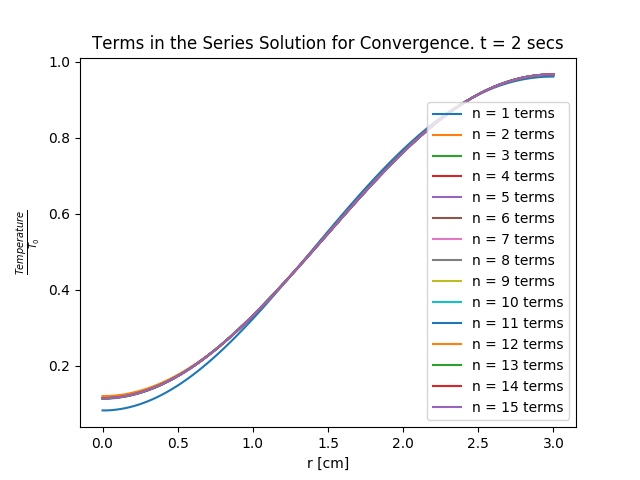
\includegraphics[scale=0.7]{terms_2.png}
  \end{center}
  \caption{Number of terms convergence study for t = 2.}
  \label{fig:2}
\end{figure}

\begin{figure}[htbp!]
  \begin{center}
    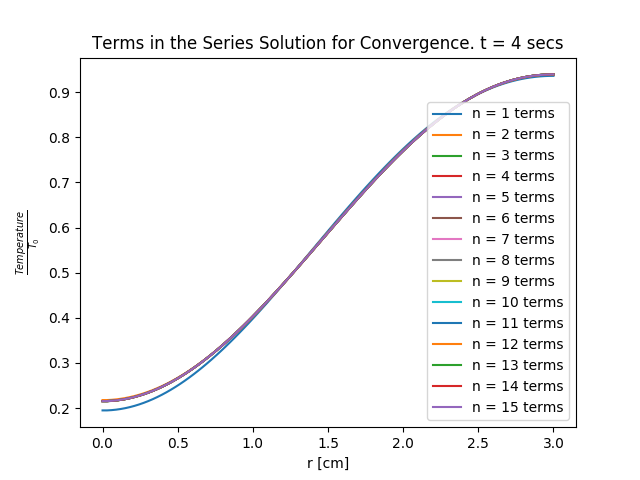
\includegraphics[scale=0.7]{terms_4.png}
  \end{center}
  \caption{Number of terms convergence study for t = 4.}
  \label{fig:4}
\end{figure}

\begin{figure}[htbp!]
  \begin{center}
    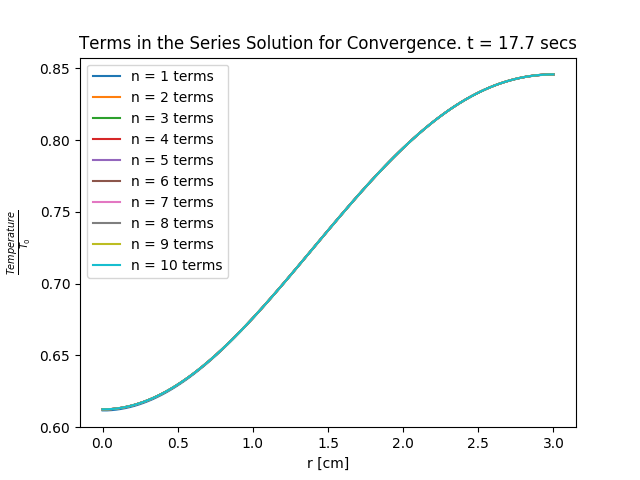
\includegraphics[scale=0.7]{terms_177.png}
  \end{center}
  \caption{Number of terms convergence study for t = 17.7.}
  \label{fig:17}
\end{figure}

\begin{figure}[htbp!]
  \begin{center}
    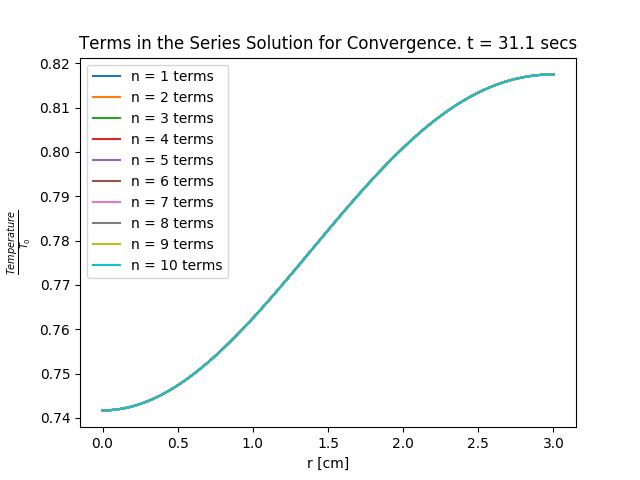
\includegraphics[scale=0.7]{terms_311.png}
  \end{center}
  \caption{Number of terms convergence study for t = 31.1.}
  \label{fig:31}
\end{figure}


\begin{figure}[htbp!]
  \begin{center}
    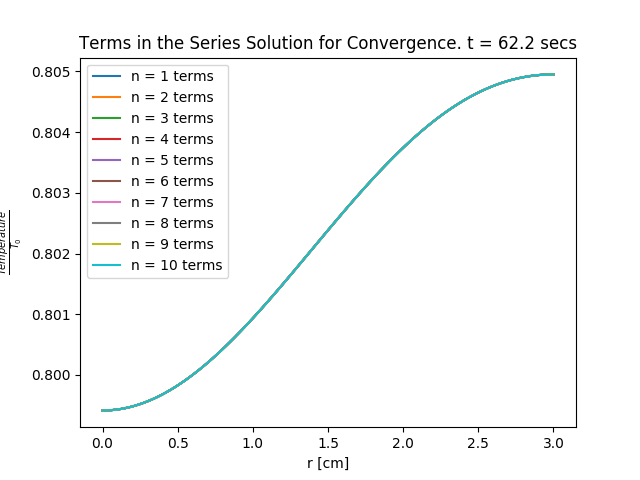
\includegraphics[scale=0.7]{terms_622.png}
  \end{center}
  \caption{Number of terms convergence study for t = 62.2.}
  \label{fig:62}
\end{figure}

\begin{figure}[htbp!]
  \begin{center}
    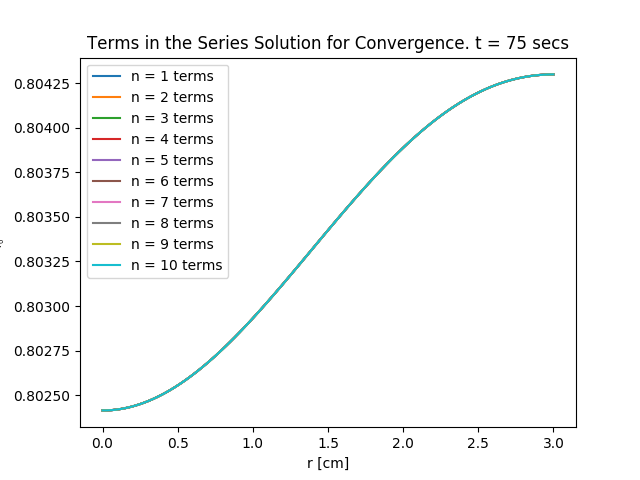
\includegraphics[scale=0.7]{terms_75.png}
  \end{center}
  \caption{Number of terms convergence study for t = 75.}
  \label{fig:75}
\end{figure}

The converged $T(r,t)$ for all seven cases is shown in \cref{fig:conv}.

\begin{figure}[htbp!]
  \begin{center}
    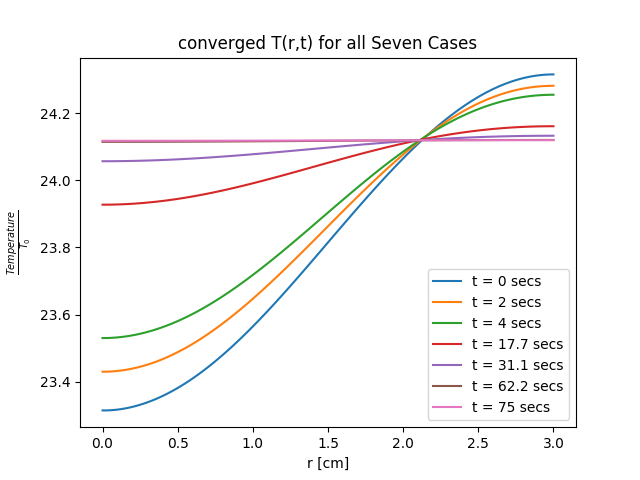
\includegraphics[scale=0.7]{converged.png}
  \end{center}
  \caption{Converged Temperature Profiles for all Seven Timesteps.}
  \label{fig:conv}
\end{figure}

Refer to appendix D for eigenvalue calculations.


\pagebreak

\section*{Numerical Solution}

Considering previous plots, it can be safely assumed that the sphere
reaches steady state after 70 seconds. Setting the maximum time to 70
seconds, the grid refinement study is done.

An important thing to note in the numerical solution is the role of
$\frac{dt}{dr}$. Varying grid size, thus varying dt and dr may cause
this term to either be close to zero or very big, which produces 
confusing results. The error depends on the ratio of the two 
terms (eg. the term will go to infinity if dr is much smaller
than dt). To prevent this from happening, only one grid size is 
changed at a time, and the other grid is set so that the $\frac{dt}{dr}$
term does not mess up the entire equation.

For the grid refinement study of spatial terms (r grid), a fixed 
time is set, and the grid size is varied. For the grid refinement
study of temporal terms (t grid), a fixed spatial grid is set
and the spatial terms are varied.

\subsection*{Spatial Grid Refinement Study}
\Cref{fig:r_10s} and \ref{fig:r_30s} show the grid refinement study
done on time 10 and 30 seconds.

\begin{figure}[htbp!]
  \begin{center}
    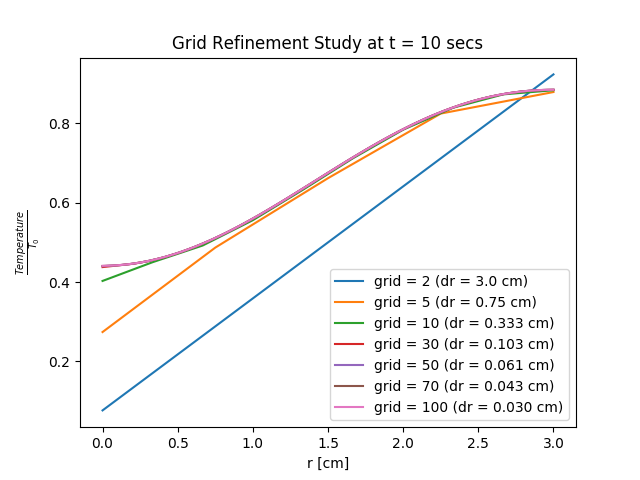
\includegraphics[scale=0.7]{grid_ref_10s.png}
  \end{center}
  \caption{Grid Refinement Study for the temperature at 10 seconds.}
  \label{fig:r_10s}
\end{figure}

\begin{figure}[htbp!]
  \begin{center}
    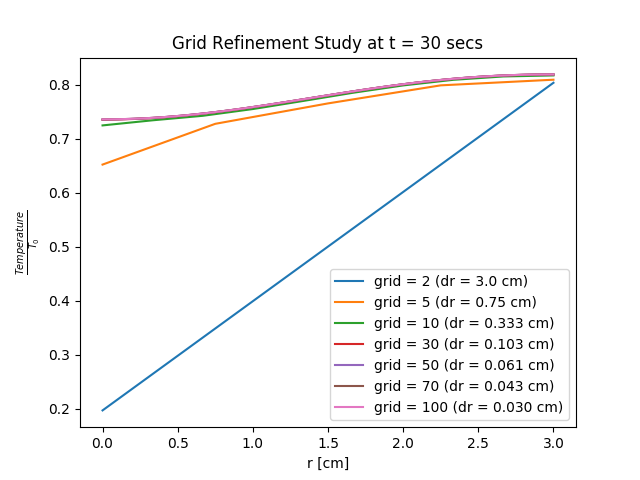
\includegraphics[scale=0.7]{grid_ref_30s.png}
  \end{center}
  \caption{Grid Refinement Study for the temperature at 30 seconds.}
  \label{fig:r_30s}
\end{figure}

With grid size under 5, the temperature profile is far from the converged.
However, when the grid size becomes larger than 15 (dr around 0.15cm),
the temperature profile converges for both timesteps. After that point,
increasing the grid size does not affect the fidelity of the temperature
profile much more, which brings the 'Goldilocks' grid size to about 20.

\subsection*{Temporal Grid Refinement Study}

With the problem with $\frac{dt}{dr}$, the r grid is set as a function
of r grid (see code for details) to prevent the equation from blowing up.
The time grid points used are 10, 50, 100 and 300, shown in \cref{fig:t_10},
\ref{fig:t_50}, \ref{fig:t_100}, \ref{fig:t_300}.


\begin{figure}[htbp!]
  \begin{center}
    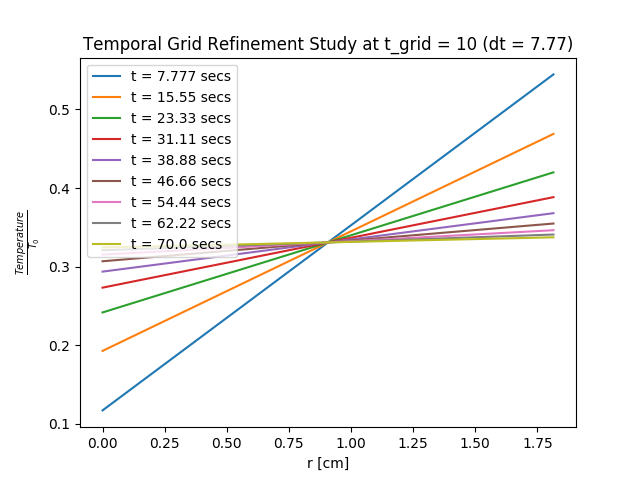
\includegraphics[scale=0.7]{t_grid_10.png}
  \end{center}
  \caption{Time Grid Refinement Study for t grid = 10}
  \label{fig:t_10}
\end{figure}


\begin{figure}[htbp!]
  \begin{center}
    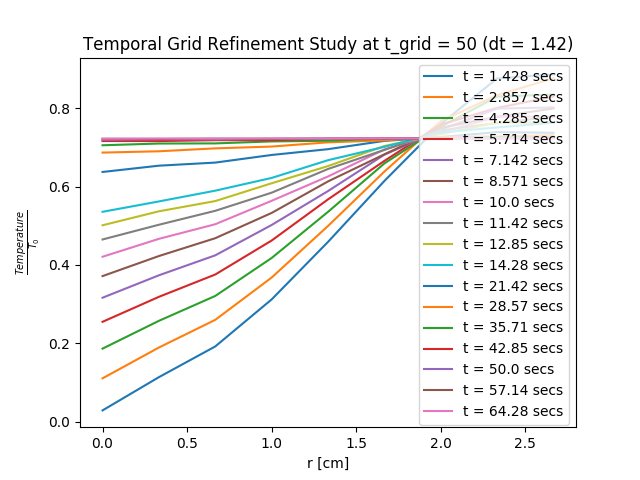
\includegraphics[scale=0.7]{t_grid_50.png}
  \end{center}
  \caption{Time Grid Refinement Study for t grid = 50}
  \label{fig:t_50}
\end{figure}


\begin{figure}[htbp!]
  \begin{center}
    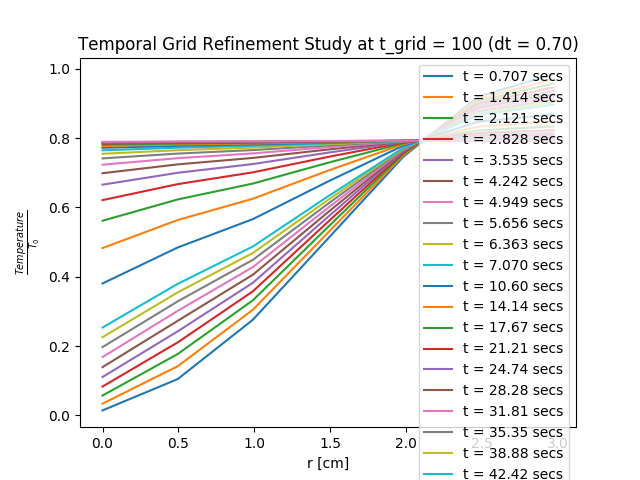
\includegraphics[scale=0.7]{t_grid_100.png}
  \end{center}
  \caption{Time Grid Refinement Study for t grid = 100}
  \label{fig:t_100}
\end{figure}


\begin{figure}[htbp!]
  \begin{center}
    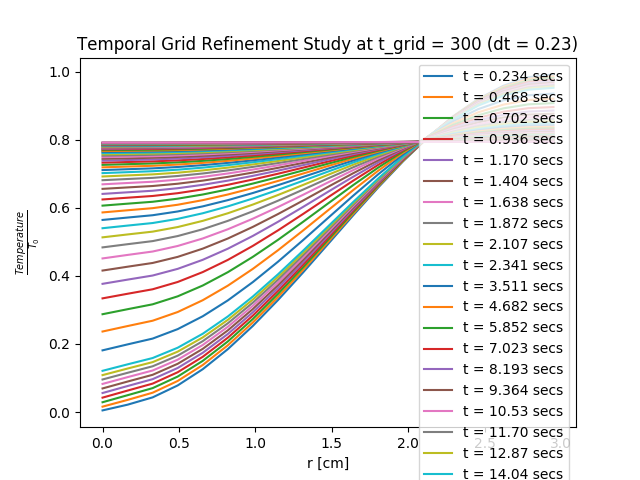
\includegraphics[scale=0.7]{t_grid_300.png}
  \end{center}
  \caption{Time Grid Refinement Study for t grid = 300}
  \label{fig:t_300}
\end{figure}

As the time grid reaches 300 (or $dt = 0.23$), the temperature profiles
are a smooth curve, like the analytical solution. Thus, it can be stated
that a time grid size of 300 is adequate for obtaining a good solution.


\subsection*{Analytical vs Numerical}
For the difference between the analytical and numerical solution,
both methods are plotted against each other in a fixed time.
The plots are in \Cref{fig:conv_2}, \ref{fig:conv_4}, \ref{fig:conv_177},
\ref{fig:conv_311}, \ref{fig:conv_622}.

\begin{figure}[htbp!]
  \begin{center}
    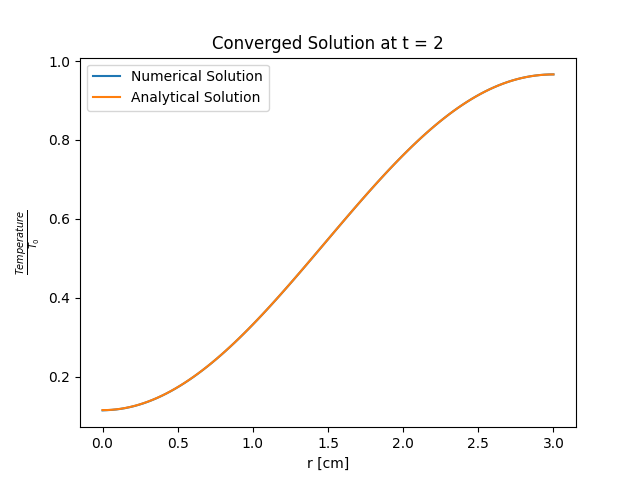
\includegraphics[scale=0.7]{conv_2s.png}
  \end{center}
  \caption{Comparison of Analytical and Numerical Solutions at t = 2s.}
  \label{fig:conv_2}
\end{figure}


\begin{figure}[htbp!]
  \begin{center}
    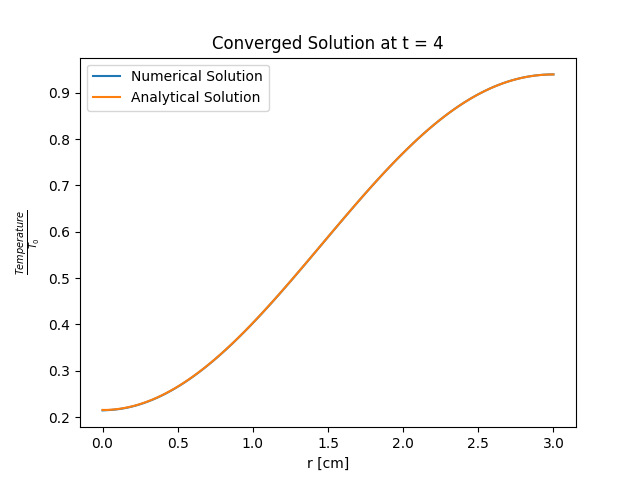
\includegraphics[scale=0.7]{conv_4s.png}
  \end{center}
  \caption{Comparison of Analytical and Numerical Solutions at t = 4s.}
  \label{fig:conv_4}
\end{figure}

\begin{figure}[htbp!]
  \begin{center}
    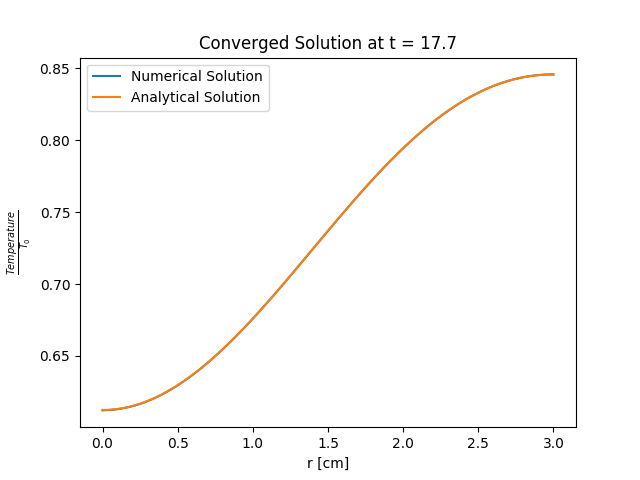
\includegraphics[scale=0.7]{conv_177s.png}
  \end{center}
  \caption{Comparison of Analytical and Numerical Solutions at t = 17.7s.}
  \label{fig:conv_177}
\end{figure}

\begin{figure}[htbp!]
  \begin{center}
    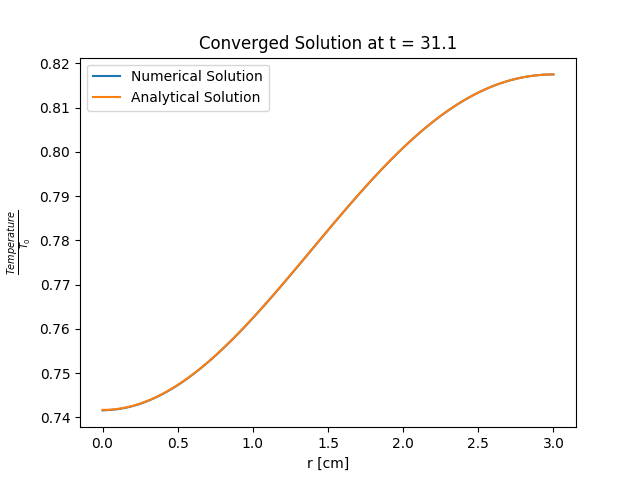
\includegraphics[scale=0.7]{conv_311s.png}
  \end{center}
  \caption{Comparison of Analytical and Numerical Solutions at t = 31.1s.}
  \label{fig:conv_311}
\end{figure}


\begin{figure}[htbp!]
  \begin{center}
    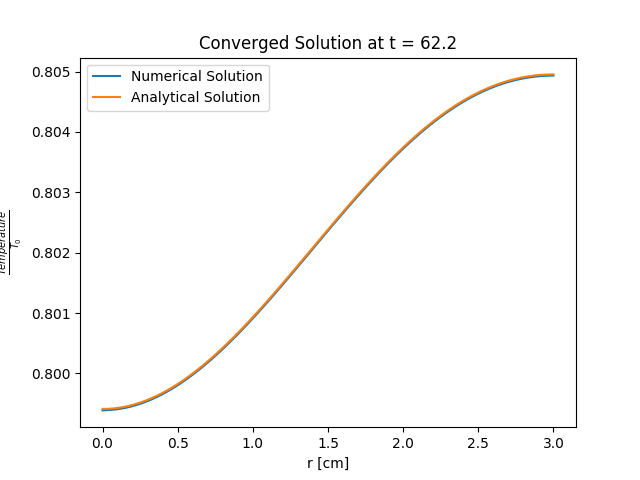
\includegraphics[scale=0.7]{conv_622s.png}
  \end{center}
  \caption{Comparison of Analytical and Numerical Solutions at t = 62.2s.}
  \label{fig:conv_622}
\end{figure}

As notably so, there is very little difference between the numerical and analytical
solution, given ample temporal and spatial grid size. 


\section*{Conclusion}
Through this exercise, a conclusion can be drawn that the numerical
and analytical solutions for the temperature profile of the sphere
has little difference. A grid refinement study is done both temporally
and spatially, to find a balance between fidelity and efficiency. 

\pagebreak
\section*{Appendix A}

\subsection*{Simple Energy Balance}
Since there is no heat generation or leakage (r=R is insulated), 
the steady state temperature is a constant throughout the sphere.

Doing a simple energy balance,

\[\frac{dE}{dt} = E_{gain} - E_{loss}\]

\[\frac{dE}{dt} = E_{gen} + E_{in} - E_{out}\]

Since there is no heat generation, flux in, or flux out (insulated BC),
the steady state is a constant temperature in time.


Expressing mathematically for when time goes to infinity:

$T_{ss}$ is when $\frac{dT}{dt} = 0 $:

\[0 = \frac{1}{r^2} \frac{d}{dr} r^2 (\frac{dT_{ss}}{dr})\]

\[\frac{C_1}{r^2} = \frac{dT_{ss}}{dr}\]

\[-\frac{C_1}{r} + C_2 = T_{ss}\]

applying BC:

at r = 0, finite, makes  $C_1 = 0$

\[T_{ss} = C_2\]

the numerical value of this constant can be found doing an energy balance
of the system with the initial condition:

\[\int_{0}^{R} \frac{T_0}{2} (1-\cos(\frac{\pi r}{R})) r^2 dr = \int_{0}^{R} C r^2 dr \]

\[\frac{T_0}{2} \int_{0}^{R}  (r^2-r^2\cos(\frac{\pi r}{R})) dr = C \frac{R^3}{3} \]

using separation of variables:

\[\frac{T_0}{2} ( \frac{R^3}{3} - (\frac{r^2 R}{\pi} \sin(\frac{\pi r}{R})\Big|_0^R - \frac{2R}{\pi} \int_0^R r \sin(\frac{\pi r}{R})))dr = C \frac{R^3}{3}\]

Solving this:

\[\frac{T_0}{2} (\frac{R^3}{3} + \frac{2R^3}{\pi ^2}) = C \frac{R^3}{3} \]

\centering{
    \mathcolorbox{yellow}{
    C = T_{ss} = \frac{3T_0}{2} (\frac{\pi^2 + 6}{3\pi^2}) \approx 0.804 T_0
}

The steady state is plotted in figure \cref{fig:ss}.

\begin{figure}[htbp!]
  \begin{center}
    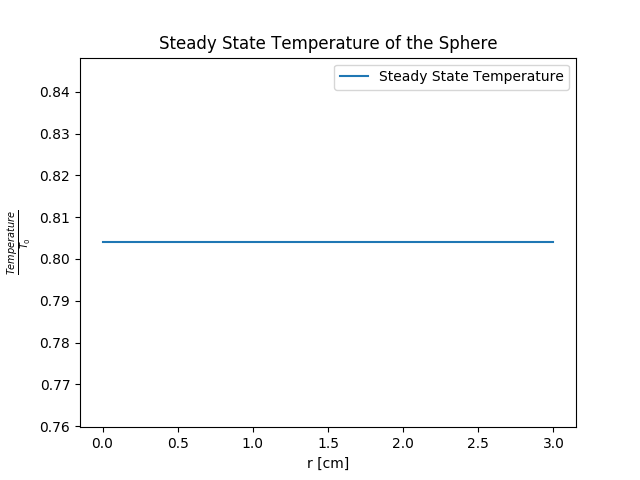
\includegraphics[scale=0.7]{steady_state.png}
  \end{center}
  \caption{Plot of Steady State Solution for the Sphere.}
  \label{fig:ss}
\end{figure}


\subsection*{Sketch of Different Temperature Profiles in Time}
The time evolution of the temperature profile starts from t=0,
with the two boundary points, $T(0,0) = 0$ and $T(R,0) = T_0$.
Through time, the temperature profile flattens out, since the 
only thing affecting the profile is heat diffusion. The steady
state (as time goes to infinity) becomes a constant throughout space.
A sketch is made in \Cref{fig:sketch}.

\begin{figure}[htbp!]
  \begin{center}
    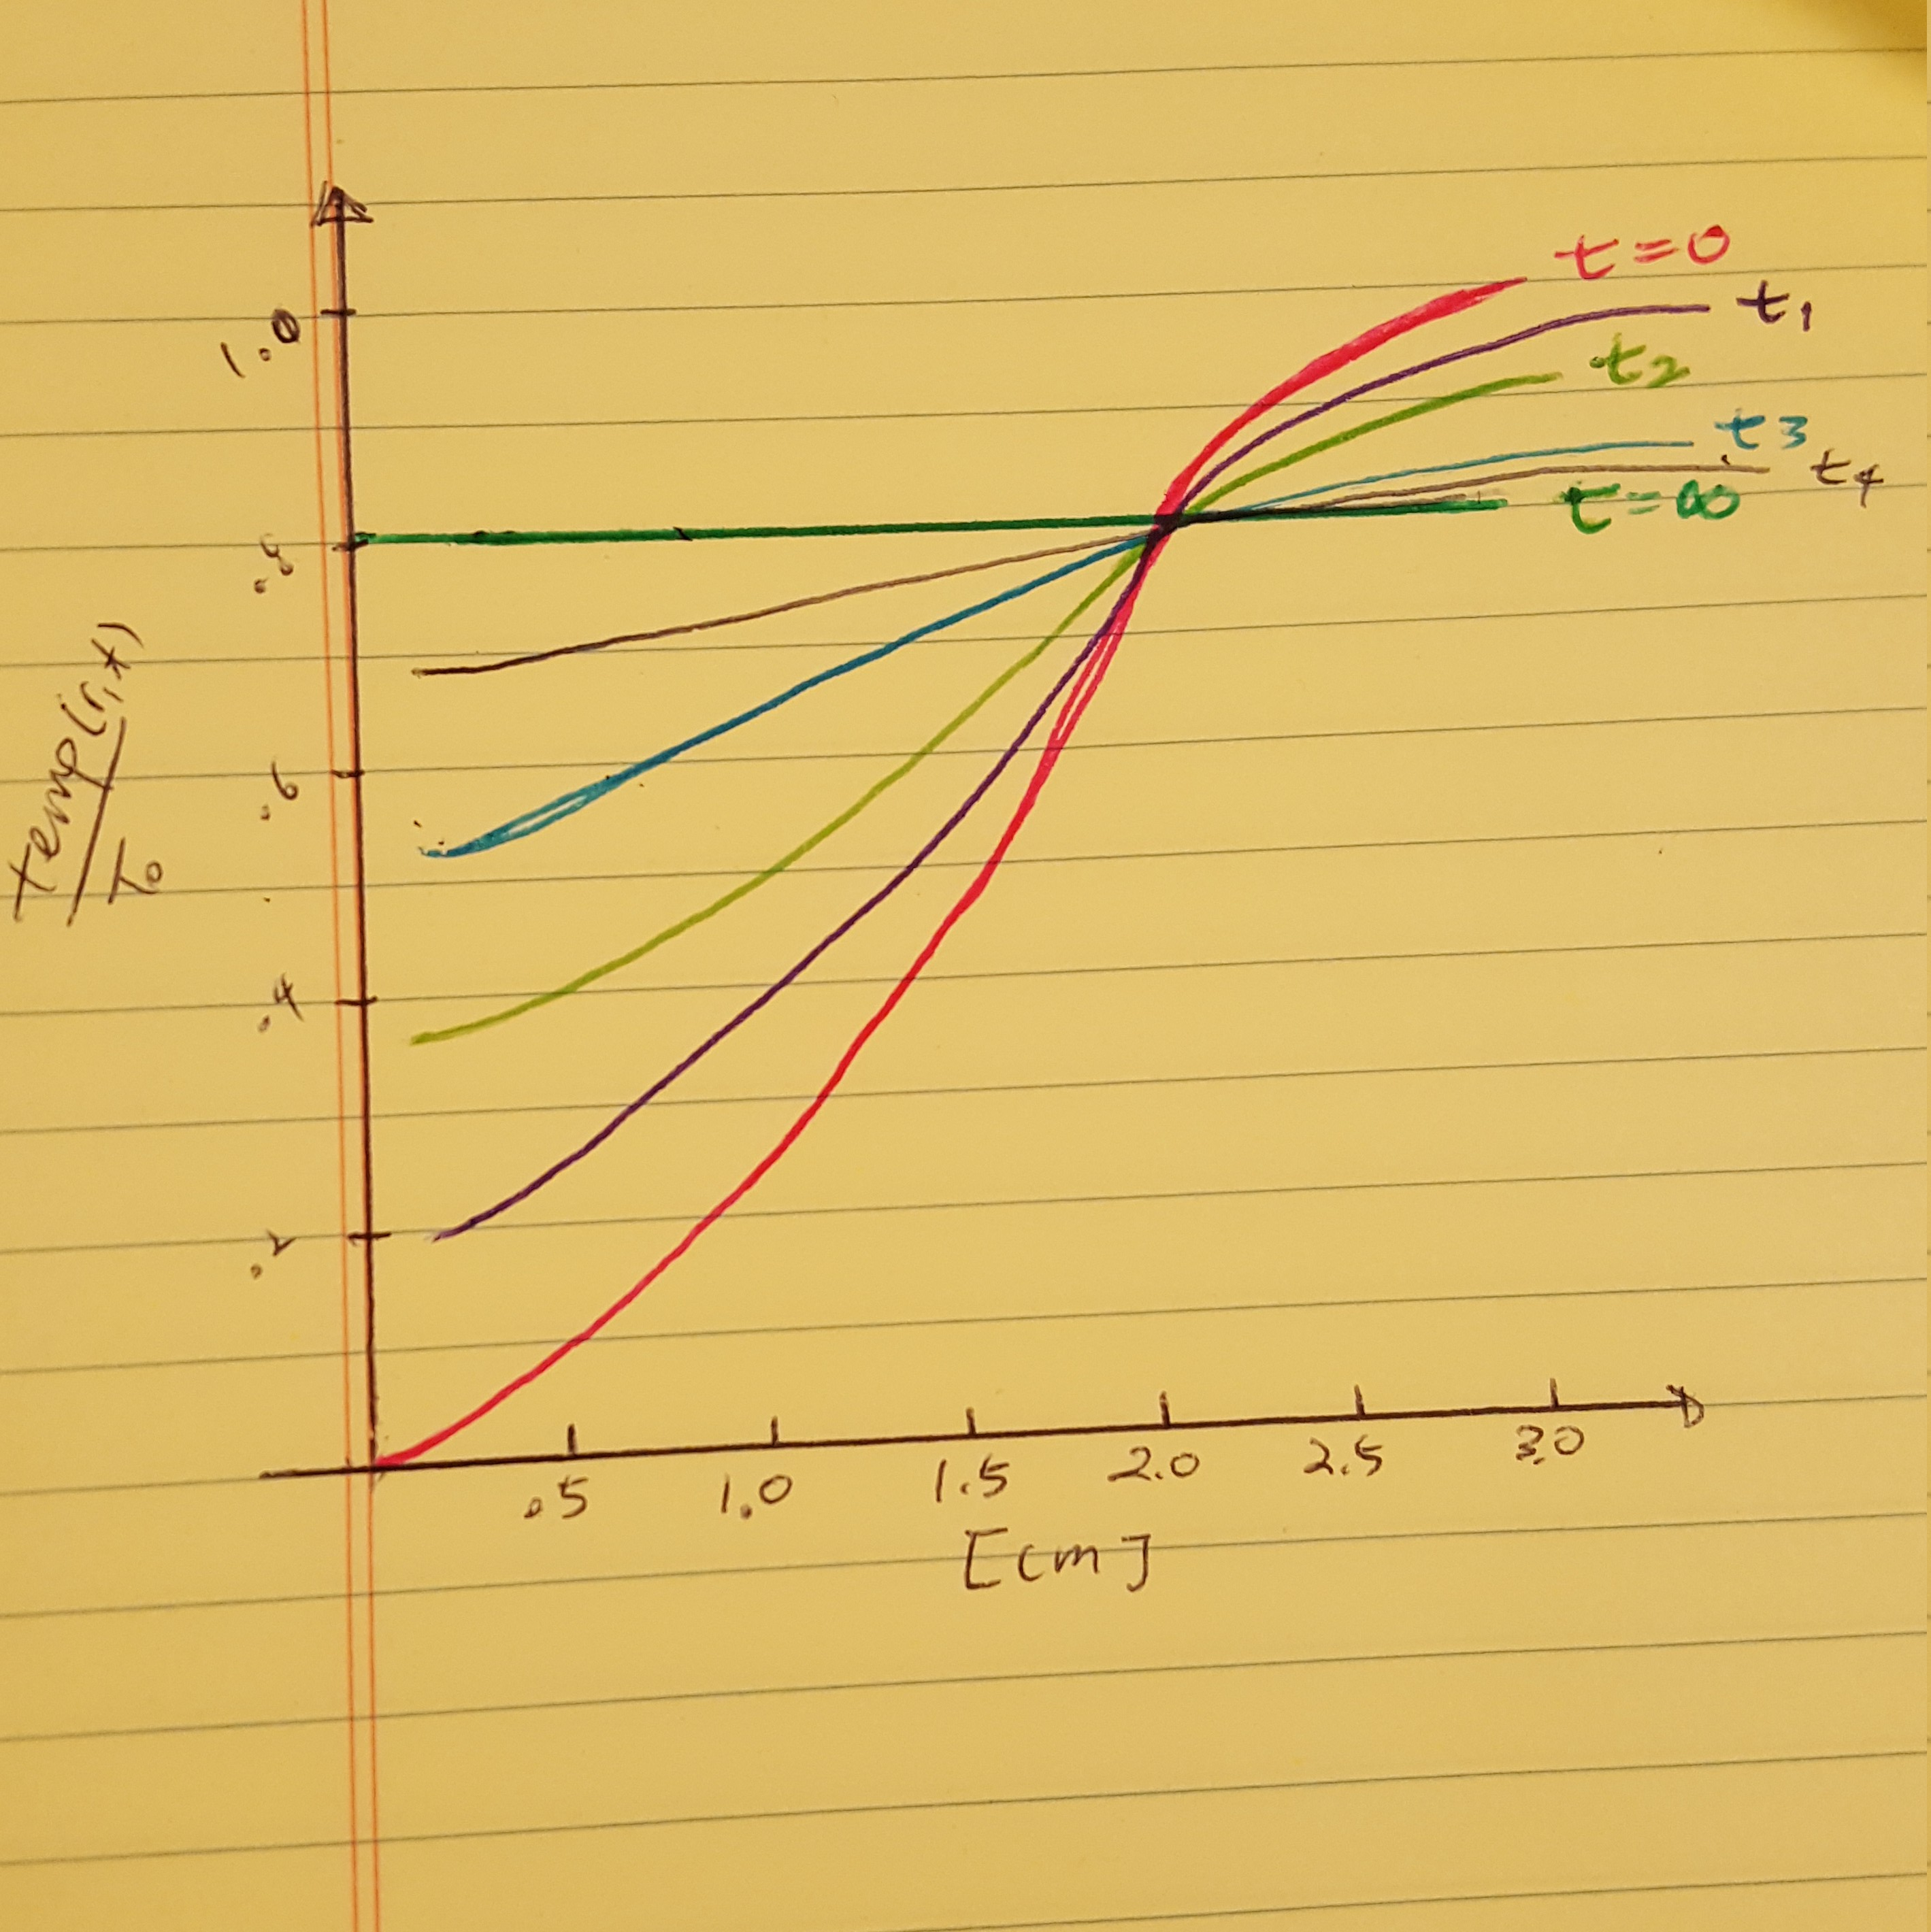
\includegraphics[width=0.6\textwidth ]{s.jpg}
  \end{center}
  \caption{Sketch of Temperature profile over time.}
  \label{fig:sketch}
\end{figure}


\section*{Solution of $T(r,t)$ for $t > 0$}
Since the numerical value of $T_{ss}$ has been found
through the energy balance, that can be added to the solution
for $T(r,t)$ for $t>0$.

The application and solution for $T(r,t)$ is shown in Appendix B.

\pagebreak
\section*{Appendix B}

\subsection*{Analytical solution for solving T(r,t) directly}

\[\frac{1}{\alpha} \cdot \frac{dT}{dt} = \frac{1}{r^2} \frac{d}{dr} r^2 \frac{dT}{dr}\]

Boundary Conditions:
\[T(0,t) = finite \]
\[\frac{dT}{dr} (r = R) = 0 \]

Initial Condition:
\[T(r,0) = \frac{T_0}{2} (1-\cos{(\frac{\pi \cdot r}{R})}) \]

set:
\[T(r,t) = \frac{\overline{T} (r,t)}{r} +T_ss\]
\[\overline{T} (r,t) = T(r,t) r + T_ss r\]

plugging this back into the differential equation:

\[\frac{1}{\alpha} \cdot \frac{d\overline{T}}{dt} \frac{1}{r} = \frac{1}{r^2} \frac{d}{dr} r^2 (\frac{d\overline{T}}{dr} \frac{1}{r} - \frac{1}{r^2} \overline{T}) \]

\[\frac{1}{\alpha} \cdot \frac{d\overline{T}}{dt} = \frac{1}{r} \frac{d}{dr} (\frac{d\overline{T}}{dr} r - \overline{T}) \]

\[\frac{1}{\alpha} \cdot \frac{d\overline{T}}{dt} = \frac{1}{r} (\frac{d^2\overline{T}}{dr^2} r + \frac{d\overline{T}}{dr} - \frac{d\overline{T}}{dr}) \]

\[\frac{1}{\alpha} \cdot \frac{d\overline{T}}{dt} = \frac{d^2\overline{T}}{dr^2} \]

where 
\[\overline{T}(0,t) = 0 \]
\[\frac{d\overline{T}}{dr} = \frac{\overline{T}}{R}\]
and initial condition
\[\overline{T} (r,0) = r \frac{T_0}{2} (1- cos(\frac{\pi r}{R})) - T_{ss} r\]

This turns into a cartesian problem.

Applying Separation of Variables:
\[\overline{T}(r,t) = \Gamma (t) \Psi (r)  \]

Applying the new variables, dividing both sides by $\Gamma (t) \Psi (r) $,
and setting it to a new variable $ -\beta^2 $:
\[\frac{1}{\alpha  \Gamma} \cdot \frac{d\Gamma}{dt} = \frac{d^2 \Psi}{dr^2} \frac{1}{\Psi} = -\beta^2 \] 

Solving for $\Psi$ first:
\[\frac{d^2 \Psi}{dr^2} \frac{1}{\Psi} = -\beta^2 \]

\[\frac{d^2 \Psi}{dr^2} + \beta^2 \Psi = 0 \]

\[\Psi (r) = C_1 sin(\beta r) + C_2 cos(\beta r) \]

Boundary Conditions:

Since:
\[\frac{dT}{dr} = -\frac{\overline{T}}{r^2} + \frac{1}{r} \frac{d\overline{T}}{dr}\]

The boundary conditions become:
\[-\Psi(r=0) = 0 \]
\[-k (\frac{\Psi}{R^2} + \frac{d\Psi}{dr} \frac{1}{R}) = 0  \]

Applying the first boundary condition,
interpreting as $\Psi(r=0) = 0 , C_2 = 0$

Applying the second boundary condition,
\[-\frac{C_1 \sin(\beta R)}{R^2} + C_1 \cos(\beta r) \beta = 0 \]
\[-\sin(\beta R) + R \beta \cos{\beta R} =0 \]
\[\tan(\beta R ) = R\beta \]


\begin{figure}[htbp!]
  \begin{center}
    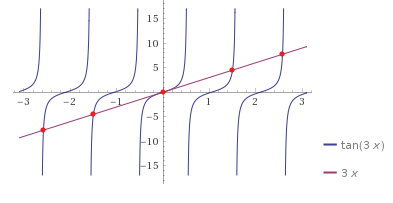
\includegraphics[scale=0.7]{tan_plot.png}
  \end{center}
  \caption{Plot of tan(3x) = 3x.}
  \label{fig:tan_plot}
\end{figure}

$\beta$ is the zeros of that equation (illustrated in \cref{fig:tan_plot})

Solving for $\Gamma(t)$:
\[\frac{1}{\alpha  \Gamma} \cdot \frac{d\Gamma}{dt} = -\beta_n^2 \]
\[\frac{1}{\alpha  \Gamma} \cdot \frac{d\Gamma}{dt} = -\beta_n^2 \alpha \Gamma \]

\[\Gamma(t) = A_1 e^{-\alpha \beta_n^2 t }\]

This makes $\overline{T}(r,t)$:

\centering{
    \mathcolorbox{yellow}{
\overline{T}(r,t) = \sum_{n=1}^{\infty} A_n e^{-\alpha \beta_n^2 t} sin(\beta_n r)
}


Applying initial condition and orthogonality:
\[T\sum_{n=1}^{\infty} A_n \sin(\beta_n r) = r \frac{T_0}{2} (1-\cos(\frac{\pi r}{R})) - T_{ss} r\]

\centering{
  \mathcolorbox{yellow}{
  A_n = \frac{\int_{0}^{R} (r \frac{T_0}{2} (1- \cos(\frac{\pi r}{R})) - T_{ss}r) \sin(\beta_n r) dr }
              {\int_{0}^{R} (\sin(\beta_n r))^2 dr}
  }
}

Plugging all this into $T(r,t)$:

\centering{
  \mathcolorbox{yellow}{
T(r,t) = \sum_{n=1}^{\infty} A_n \frac{\sin(\beta_n r)}{r} e^{-\beta_n^2 \alpha t} + T_{ss}
  }
}



\subsection*{Analytical solution by defining new temperature}

\[T'(r,t) = T(r,t) - T_{ss}\]

\[T'(r,t) + T_{ss} = T(r,t) \]


where $T_{ss}$ is:


\[0 = \frac{1}{r^2} \frac{d}{dr} r^2 (\frac{dT_{ss}}{dr})\]

\[\frac{C_1}{r^2} = \frac{dT_{ss}}{dr}\]

\[-\frac{C_1}{r} + C_2 = T_{ss}\]

applying BC:

at r = 0, finite, makes  $C_1 = 0$

\[T_{ss} = C_2\]

Plugging the new definition into the original differential equation:

differential equation becomes:

\[\frac{1}{\alpha} (\frac{dT'}{dt} + \frac{dT_{ss}}{dt}) = \frac{1}{r^2} \frac{d}{dr} r^2 (\frac{dT'}{dr} + \frac{dT_{ss}}{dr})\]

Considering $\frac{dT_{ss}}{dt} = \frac{dT_{ss}}{dr} = 0$,

\[\frac{1}{\alpha} \cdot \frac{dT'}{dt} = \frac{1}{r^2} \frac{d}{dr} r^2 \cdot \frac{dT'}{dr} \]

Boundary Conditions
\[T'(0,t)  = finite \]
\[\frac{dT'}{dr} (r = R) = 0 \]

Initial Condition:
\[T'(r,0) = \frac{T_0}{2} (1-\cos{(\frac{\pi \cdot r}{R})}) - C_2 \]

set:
\[T'(r,t) = \frac{\overline{T'}}{r} \]


\[\frac{1}{\alpha} \cdot \frac{d\overline{T'}}{dt} \frac{1}{r} = \frac{1}{r^2} \frac{d}{dr} r^2 (\frac{d\overline{T'}}{dr} \frac{1}{r} - \frac{1}{r^2} \overline{T'}) \]

\[\frac{1}{\alpha} \cdot \frac{d\overline{T'}}{dt} = \frac{1}{r} \frac{d}{dr} (\frac{d\overline{T'}}{dr} r - \overline{T'}) \]

\[\frac{1}{\alpha} \cdot \frac{d\overline{T'}}{dt} = \frac{1}{r} (\frac{d^2\overline{T'}}{dr^2} r + \frac{d\overline{T'}}{dr} - \frac{d\overline{T'}}{dr}) \]

\[\frac{1}{\alpha} \cdot \frac{d\overline{T'}}{dt} = \frac{d^2\overline{T'}}{dr^2} \]

turns into a cartesian problem.

Applying Separation of Variables:
\[\overline{T'}(r,t) = \Gamma (t) \Psi (r)  \]

Boundary Conditions:

\[\Psi(r = 0) = finite \]
\[\frac{d\Psi}{dr} (r = R) = 0 \]

Applying the new variables, dividing both sides by $\Gamma (t) \Psi (r) $,
and setting it to a new variable $ -\beta^2 $:
\[\frac{1}{\alpha  \Gamma} \cdot \frac{d\Gamma}{dt} = \frac{d^2 \Psi}{dr^2} \frac{1}{\Psi} = -\beta^2 \] 

Solving for $\Psi$ first:
\[\frac{d^2 \Psi}{dr^2} \frac{1}{\Psi} = -\beta^2 \]

\[\frac{d^2 \Psi}{dr^2} + \beta^2 \Psi = 0 \]

\[\Psi (r) = C_1 sin(\beta r) + C_2 cos(\beta r) \]

Applying the first boundary condition,
interpreting as $\Psi(r=0) = 0 , C_2 = 0$

Applying the second boundary condition,
\[-\frac{C_1 \sin(\beta R)}{R^2} + C_1 \cos(\beta r) \beta = 0 \]
\[-\sin(\beta R) + R \beta \cos{\beta R} =0 \]
\[\tan(\beta R ) = R\beta \]

$\beta$ is the zeros of that equation.

Solving for $\Gamma(t)$:
\[\frac{1}{\alpha  \Gamma} \cdot \frac{d\Gamma}{dt} = -\beta_n^2 \]
\[\frac{1}{\alpha  \Gamma} \cdot \frac{d\Gamma}{dt} = -\beta_n^2 \alpha \Gamma \]

\[\Gamma(t) = A_1 e^{-\alpha \beta_n^2 t }\]

This makes $\overline{T'}(r,t)$:
\[\overline{T'}(r,t) = A_n e^{-\alpha \beta_n^2 t} sin(\beta_n r)\]

Solving back for $T'(r,t)$:
\[T'(r,t) = \frac{A_n}{r} e^{-\alpha \beta_n^2 t} sin(\beta_n r)\]

Applying initial condition and orthogonality:
\[T'(r,0) = \frac{A_n}{r} sin(\beta_n r) = \frac{T_0}{2} (1-\cos{(\frac{\pi \cdot r}{R})}) + C_2\]

\[A_n = \frac{\int_{0}^{R}  r^3 sin(\beta_n r) (\frac{T_0}{2} \cdot (1-\cos{\frac{\pi r}{R}}) + C_2) dr} {\int_{0}^{R} r^2 \sin^2{\beta_n r} dr }\]

The analytical solution is:
\[T'(r,t) = \frac{\int_{0}^{R}  r^3 sin(\beta_n r) (\frac{T_0}{2} \cdot (1-\cos{\frac{\pi r}{R}}) + T_{ss}) dr} {\int_{0}^{R} r^2 \sin^2{\beta_n r} dr } e^{-\alpha \beta_n^2 t} sin(\beta_n r)\]

\[T = \frac{\int_{0}^{R}  r^3 sin(\beta_n r) (\frac{T_0}{2} \cdot (1-\cos{\frac{\pi r}{R}}) + T_{ss}) dr} {\int_{0}^{R} r^2 \sin^2{\beta_n r} dr } e^{-\alpha \beta_n^2 t} sin(\beta_n r) + T_{ss} \]

Since the solution from the previous question with $n=0$ covers the 
steady state case, this problem is redundant and provides
no new insight into the problem.

\section*{Appendix D - Eigenvalues}

The eigenvalues are acquired by a script that assesses zero
points from the equation:
\begin{minted}{python}
import numpy as np


def beta_equation(beta):
    y = 3*beta - np.tan(beta * 3)
    return y 

R = 3
k = 0.15
rho = 8000. / 1000000.
cp = 500
alpha = k / (rho*cp)
T_0 = 1

points = np.arange(0, 1e2, 1e-5)
pot_betas = []
count = 0
flag = 1
for beta in points:
    if beta_equation(beta) > 0:
        flag = 0
    elif beta_equation(beta) < 0 and flag == 0:
        pot_betas.append(beta)
        count = count + 1
        flag = 1
betas = pot_betas

\end{minted}

The acquired eigenvalues are listed in \cref{tab:eign}. Only the first
25 terms are shown for brevity.

\begin{table}[h]
     \centering
    \begin{tabularx}{\textwidth}{bb}
       \hline
       \textbf{Term Number ($n$)} & \textbf{Eigenvalue ($\beta_n$)}  \\
       \hline
        0 & 0 \\
        1 & 1.49781\\ 
        2 & 2.57509\\ 
        3 & 3.63471\\ 
        4 & 4.68874\\ 
        5 & 5.74026\\ 
        6 & 6.79044\\ 
        7 & 7.83982\\ 
        8 & 8.88869\\ 
        9 & 9.9372\\ 
        10 & 10.98547\\ 
        11 & 12.03355\\ 
        12 & 13.08148\\ 
        13 & 14.12931\\ 
        14 & 15.17705\\ 
        15 & 16.22472\\ 
        16 & 17.27233\\ 
        17 & 18.3199\\ 
        18 & 19.36742\\ 
        19 & 20.41492\\ 
        20 & 21.46238\\ 
        21 & 22.50982\\ 
        22 & 23.55723\\ 
        23 & 24.60463\\ 
        24 & 25.65201\\ 
        25 & 26.69938\\ 

        \hline
    \end{tabularx}
    \caption {First 25 eigenvalues acquired.}
    \label{tab:eign}
\end{table}





\section*{Appendix D - Numerical Solution}


\[\frac{1}{\alpha} \cdot \frac{dT}{dt} = \frac{2}{r} \frac{dT}{dr} + \frac{d^2T}{dr^2}\]

Applying the finite difference method, central for r and explicit for t:
\[\frac{1}{\alpha} \cdot \frac{T_k^{u} - T_k^{u-1}}{\Delta t} = \frac{2}{r_k} \; (\frac{T^{u-1}_{k+1}-T^{u-1}_{k-1}}{2 \Delta r}) + \frac{T^{u-1}_{k-1} - 2T^{u-1}_k + T^{u-1}_{k+1}}{\Delta r^2}\]

where u is the temporal step and k is the spacial step.

Solving for $T_{k}^{u+1}$:

\centering{
    \mathcolorbox{yellow}{
    T_{k}^{u+1} = T_k^u + \alpha \frac{\Delta t }{\Delta r \cdot r} (T_{k+1}^u + T_{k-1}^u) + \alpha * \frac{\Delta t}{(\Delta r)^2} (T_{k+1}^{u} -2T_k^u + T_{k-1}^u) }
}


Applying neuman boundary condition at r=0:
\[\frac{dT(0,t)}{dr} =0 \]
\[\frac{T_1^u - T_{-1}^u}{2\Delta r} =0 \]
\[T_1^u = T_{-1}^u\]

This gives:

\centering{
    \mathcolorbox{yellow}{T_0^{u+1} = T_0^u + \alpha * \frac{\Delta t}{(\Delta r)^2} (2T_{1}^{u} -2T_0^u ) }
}


Applying neuman boundary condition at r=R (k=K at r=R):
\[-k \frac{dT(R,t)}{dr} =0 \]
\[\frac{T_{K+1}^u - T_{K-1}^u}{2\Delta r} =0 \]
\[T_{K+1}^u = T_{K-1}^u\]

This gives:

\centering{
    \mathcolorbox{yellow}{T_K^{u+1} = T_K^u + \alpha * \frac{\Delta t}{(\Delta r)^2} (2T_{K-1}^{u} -2T_K^u )}
}


\subsection*{Numerical Solution Code}
\begin{minted}{python}

def numerical (r_grid, t_max):
    # GRID AND STUFF 
    R = 3
    k = 0.15
    rho = 8000. / 1000000.
    cp = 500
    alpha = k / (rho*cp)
    T_0 = 1

    t_grid = 1000

    r_list = np.linspace(0, R, r_grid) 
    dr = r_list[1] - r_list[0]
    t_list = np.linspace(0, t_max, t_grid)
    dt = t_list[1] - t_list[0]

    if dt/dr > 1e8:
        raise ValueError('Too high of dt/dr dude')  

    t = np.zeros((len(r_list), len(t_list)), dtype=float)

    # Apply Initial Condition
    t[:,0] = (T_0 / 2) * (1 - np.cos(np.pi * r_list / R))
    print(t[:,0])

    x = dt/dr
    
    plt.plot(r_list, t[:,0], label='t = 0 secs')

    for timestep in range(1, len(t_list)):
        t[0,timestep] = t[0,timestep-1] + (alpha * (x/dr) * (2*t[1,timestep-1] - 2*t[0,timestep-1]))
        t[-1,timestep] = t[-1, timestep-1] + alpha * (x/dr) * (2*t[-2,timestep-1] - 2*t[-1,timestep-1])
        for space in range(1, len(r_list)-1):
            first_term = alpha * (x/r_list[space]) * (t[space+1,timestep-1] - t[space-1, timestep-1])
            second_term = alpha * (x/dr) * (t[space+1, timestep-1] - (2*t[space, timestep-1]) + t[space-1, timestep-1])
            t[space, timestep] = t[space, timestep-1] + first_term + second_term

        if timestep%100 ==0:
            plt.plot(r_list, t[:,timestep], label='t = %s secs' %str(t_list[timestep])[:5])

    print(t)
    plt.ylabel(r'$\frac{Temperature}{T_0}$')
    plt.xlabel('r [cm]')
    plt.legend()
    plt.title('Numerical Solution of Time-evolution of Heat Profile')
    plt.savefig('Numerical.png', format='png')
    plt.show()

\end{minted}


\subsection*{Analytical Solution Code}
\begin{minted}{python}
def analytical (r_grid, t_max, t_grid, n):
    R = 3
    k = 0.15
    rho = 8000. / 1000000.
    cp = 500
    alpha = k / (rho*cp)
    T_0 = 1

    #########################
    # finding betas
    points = np.arange(-0.1, 1e3, 1e-4)
    pot_betas = []
    for beta in points:
        if beta_equation(beta) > 0:
            flag = 0
        elif beta_equation(beta) < 0 and flag == 0:
            pot_betas.append(beta)
            flag = 1

    # pick only first n betas
    betas = pot_betas[:n]
    print(betas)
    ###########################

    T_0 = 1
    r_list = np.linspace(0, R, r_grid)
    dr = r_list[1] - r_list[0]
    t_list = np.linspace(0, t_max, t_grid)
    dt = t_list[1] - t_list[0]

    t = [0] * r_grid
    t_compiled_betas = [0] * r_grid
    t_tot = (T_0 / 2) * (1 - np.cos(np.pi * r_list / R))
    t_ss = 3*T_0 /2 * ((np.pi**2 + 6)/(3*np.pi**2))
    print(t_ss)
    steady_state = [t_ss] * r_grid
    # plot initial condition
    plt.plot(r_list, t_tot, label = 't = 0 secs')
    plt.plot(r_list, steady_state, label = 'Steady State')

    def integrand1(r, b, T_0, R, t_ss):
        return ((r*T_0*0.5*(1-np.cos(np.pi*r / R)) - t_ss * r)*np.sin(b * r))
    def integrand2(r, b):
        return ((np.sin(b*r))**2) 

    print(betas)
    for time in range(1, len(t_list)):
        t_compiled_betas = [0] * r_grid
        for b in betas[1:]:
            t = [0] * r_grid
            for space in range(1, len(r_list)):
                r = r_list[space]
                integral1 = integrate.quad(integrand1, 0, R, args=(b, T_0, R, t_ss))
                integral2 = integrate.quad(integrand2, 0, R, args=(b))
                a = integral1[0] / integral2[0]
                spatial = np.sin(b*r) / r
                temporal = np.exp(-1 * b**2 * alpha * t_list[time])
                t[space] = a * spatial * temporal
                t[0] = t[1]
            t_compiled_betas = [x+y for x,y in zip(t_compiled_betas, t)]

        t_compiled_betas = [x+t_ss for x in t_compiled_betas]    
        plt.plot(r_list, t_compiled_betas, label='t = %s secs' %str(t_list[time])[:5])
        t_tot = np.vstack((t_tot, t_compiled_betas))

    print(t_tot)
    plt.ylabel(r'$\frac{Temperature}{T_0}$')
    plt.xlabel('r [cm]')
    plt.legend()
    plt.title('Analytical Solution of Time-evolution of Heat Profile')
    plt.savefig('Analytical.png', format='png')
    plt.show()
\end{minted}

\pagebreak

-end of report.
\end{document}






